\documentclass[11pt]{article}

\usepackage[UTF8]{ctex} % for Chinese 

\usepackage{setspace}
\usepackage[colorlinks,linkcolor=blue,anchorcolor=red,citecolor=black]{hyperref}
\usepackage{lineno}
\usepackage{booktabs}
\usepackage{graphicx}
\usepackage{float}
\usepackage{floatrow}
\usepackage{subfigure}
\usepackage{caption}
\usepackage{subcaption}
\usepackage{geometry}
\usepackage{multirow}
\usepackage{longtable}
\usepackage{lscape}
\usepackage{booktabs}
\usepackage{natbib}
\usepackage{natbibspacing}
\usepackage[toc,page]{appendix}
\usepackage{makecell}

\title{孔子}
\date{}

\linespread{1.5}
\geometry{left=2cm,right=2cm,top=2cm,bottom=2cm}

\begin{document}

  \maketitle
  
  \begin{figure}[H]
    \centering
    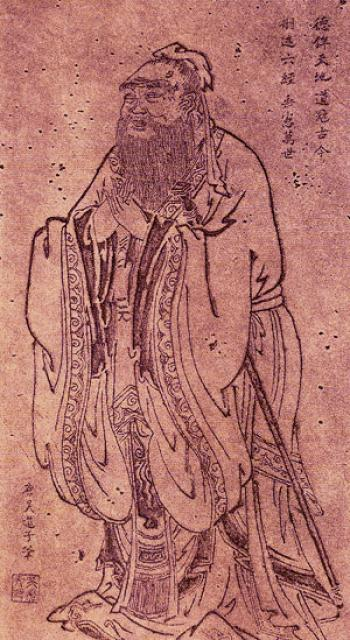
\includegraphics[height=\textwidth]{../Figures/Confucius_Tang_Dynasty.jpg}
    \caption{孔子像。唐吴道子作。}
  \end{figure}

  \newpage
  
  \linenumbers


孔子(551 BC-479 BC),名丘,字仲尼。
相传孔子先祖为宋之贵族,为殷商后人。
然孔子从周而不承殷。
殷俗重神贵卜,以巫执政,诸事皆决于鬼神,故而轻人事,生活态度放任,多驰骋于幻想世界。
先秦楚文化颇得殷商衣钵。
屈子《九歌》,犹存其风。
周人以“小邦周”推翻“大邑商”,初期局势尚不稳定。
成王之时,殷人叛乱,管蔡倒戈。
当此危急之时,周人不得不作存亡之争。
欲作艰苦奋斗,则必须在思想文化上肯定人自身之力量,即坚信人自身之努力足以克服客观存在之困难。
由此,周文化有肯定人之主宰地位的思想倾向。
周之建国,以制度为重,一面封邦建国,以一人为的政治秩序代替部落酋长式的自然秩序;一面立宗法制度,将血缘人伦纳入政治关系。
此等举措,本意是建立一强有力的中央政府,加强对地方的控制;却暗含对人事的重视,肯定人之地位,极大地削弱对鬼神巫卜的依赖。
此种事实所暗示的思想倾向由孔子明确指出并形成确定理论,遂为中华文明之精义。

\newline

\section{礼仪之辩}
孔子之学自礼始。
此处需就礼之概念作一澄清。
狭义之礼指具体仪式;广义之礼指人为创造之秩序。
为行文清晰,今将仪式之礼称为仪,而将秩序之礼称为礼。
礼仪之分辨,在孔子之前已有学者涉及。
如《左传·昭公五年载》:

\textit{公如晋,自郊劳至于赠贿,无失礼。晋侯谓女叔齐曰:“鲁侯不亦善于礼乎!”对曰:“鲁侯焉知礼!”公曰:“何为?自郊劳至于赠贿,礼无违者,何故不知?”对曰:“是仪也,不可谓礼。礼,所以守其国,行其政令,无失其民者也。今政令在家,不能取也。有子家羁,弗能用也。奸大国之盟,陵虐小国。利人之难,不知其私。公室四分,民食于他。思莫在公,不图其终。为国君,难将及身,不恤其所。礼这本末,将于此乎在,而屑屑焉习仪以亟。言善于礼,不亦远乎?”君子谓叔侯于是乎知礼。}

女叔齐谓“郊劳至于赠贿”为仪并视之为末节或者说表象,而以礼为根本或者说实质。
礼之作用在于“守其国,行其政令,无失其民”。
“今政令在家”至“不图其终”,言鲁侯不能妥善治理国家。
故讥其舍本逐末,不知礼而“屑屑焉习仪以亟”。
由文末“君子谓”可见,此等礼仪之分及轻仪贵礼之主张颇流行于古大夫。
至此,仪、礼之概念已明,方可论孔子之学。

\newline

\section{礼归于义}
春秋时期,礼崩乐坏,诸侯征伐不休,时局混乱不堪。
周王朝旧有秩序逐渐崩溃,而新秩序尚未建立。
面对此种混乱,孔子以恢复旧秩序,复兴周礼为己任。
《论语·八佾》载:

\textit{子曰:“周监于二代,郁郁乎文哉,吾从周。”}

孔子从周,欲复周礼。
则周礼之依据何在?
或者说,礼之根据何在?
我们所遵循,或需要遵循的秩序从何而来?
此种秩序,若无一坚实根基,自不能使之通行。

\newline

孔子之前,士大夫多将礼归于天道,即将人为创造之社会秩序归因于自然存在的某种神圣。
故守礼即是敬天,即是遵守自然秩序,即是敬重自然之神圣不可侵犯。
如《左传》文公十五年载:

\textit{齐侯侵我西鄙,谓诸侯不能也。遂伐曹,入其郛,讨其来朝也。季文子曰:“齐侯其不免乎。己则无礼,而讨于有礼者,曰:‘女何故行礼!’礼以顺天,天之道也。己则反天,而又以讨人,难以免矣。诗曰:‘胡不相畏,不畏于天?’君子之不虐幼贱,畏于天也。在周颂曰:‘畏天之威,于时保之。’不畏于天,将何能保?以乱取国,奉礼以守,犹惧不终,多行无礼,弗能在矣!”}

季文子谓礼为“天之道”。
畏天之威,故而守礼;违背天道,自不能免。
此实为上古原始宗教信仰之流变。
如此所谓的“天”,或自然,可视为宗教之人格神明,亦可视为形而上之至高。

\newline

孔子之成就便是将礼,或者说人为之秩序,从天这一原始信仰中解放,并使之依附于义。
义,即正当,正确,或应当如何,系对价值之判断。
孔子以义为礼之基础。
《论语·卫灵公》载:

\textit{子曰:君子义以为质,礼以行之,孙以出之,信以成之。君子哉。}

“质”即本质。
孔子谓,君子以义为本质,并通过遵循礼来执行义。
换言之,义为礼之根本,礼为义之表现。
故外在之社会秩序以正当性为基础,源于人要求正当性之意识,与一切历史习俗、社会事实均无干系。
由此,人的自觉意识为判断正当之依据,人之地位陡然显出。

\newline

再论仪、礼、义三者之关系。仪为末节,礼为根本,故不必拘泥于仪式。
《论语·八佾》载:

\textit{林放问礼之本,子曰:“大哉问!礼,与其奢也,宁俭;丧,与其易也,宁戚。”}

引文中的“礼”实为仪。
此种术语混淆常见于坟籍。
盖古人著书,不以构建系统性理论为纲,亦不重视术语之明确,论述之清晰。
况《论语》系孔子语录,此种不严格甚是常见。
此处孔子谓,仪式应当节俭,不必铺张浪费。
以丧礼为例,其意义在于哀悼死者。
与宏大仪式相比,参加丧礼者发自内心之悲戚,对死者之真诚哀悼更为重要。
俗语谓“心到神知,上供人吃”,即是此理。

\newline

然仪亦不可随意变更。
仪为礼之末节,而礼以义为根本。
故仪之变更当合乎礼,更要合乎义。
仪式可予以改变,但不可有损其所表现出的秩序。
故仪无需拘泥传统,亦无需顺从流俗。
如《论语·子罕》载:

\textit{子曰:“麻冕,礼也;今也纯,俭,吾从众。拜下,礼也;今拜乎上,泰也;虽违众,吾从下。”}

将麻冕换为纯(丝)冕,节省经费,无损于礼,故孔子从之。
“拜下”指臣见君时需先于堂下跪拜,以示尊敬。
于堂上跪拜,流俗以为亦可。
孔子谓此有损臣子对君主之尊敬,破坏君臣之秩序,故不从俗。

\newline

\section{摄义归仁}
秩序源于人对价值之要求,即礼归于义。
然不同人对同一事物,往往观点不同,如前引文之“拜下”。
既然如此,如何为应当,如何为不应当?
对一事物,如何判断其正确错误?
判其为义或不义之依据何在?
此价值根源问题不可不做一明确回答。
否则便无所谓正当或不正当,前述理论皆不能立。

\newline

孔子谓义之依据在于仁。
仁,即视人如己,净除私累。
《论语·雍也》载:

\textit{子贡曰:“如有博施于民而能济众,何如?可谓仁乎?”子曰:“何事于仁,必也圣乎!尧舜其犹病诸!夫仁者,己欲立而立人,己欲达而达人。能近取譬,可谓仁之方也已。”}

仁乃超越自我、人己等视之公心。
仁者立公心,无私累,则对外界事物可立一正当价值判断。
其所好者合乎义,其所恶者不合乎义。
而一般人无此境界,无法根据义判断事物。
此等境界,乃一自觉境界,不假外求,不受制约,以人之自主为最终主宰。
故《论语·述而》载:

\textit{子曰:“仁远乎哉?我欲仁,斯仁至矣。”}

此即强调仁之自觉性。
换言之,人能否作出正当价值判断系一自主意志问题,而非对价值了解之问题,即与具体知识无关。

\newline

为达成仁之境界,要求人在实践中视人如己,诚敬不苟,不为利欲所支配,不侵人以自利。
此类实践称为恕。
《论语·颜渊》载:

\textit{仲弓问仁。子曰:“出门如见大宾,使民如承大祭。己所不欲,勿施于人。在邦无怨,在家无怨。”仲弓曰:“雍虽不敏,请事斯语矣。”}

《卫灵公》又载:

\textit{子贡问曰:“有一言而可以终身行之者乎?”子曰:“其恕乎!己所不欲,勿施于人。”}

恕系达成仁之境界所需之训练。
换言之,需经过恭慎不苟、诚信无妄、视人如己等诸多实践训练,方能去私立公,达到仁之境界。

\section{正名}
孔子之学,其最初目的为恢复周王朝旧有秩序,结束列国纷争之混乱,故其理论最终仍需落脚于政治。
其政治思想,以正名为主。

\newline

正名,即依照各人之身份,划定其权利义务。
有君之名者,需完成君之义务,且只可享有君之权利;
为臣者,需完成臣之义务,且只可享有臣之权利。
《论语·颜渊》载:

\textit{齐景公问政于孔子。孔子对曰:“君君,臣臣,父父,子子。”}

此处孔子谓,有“君”之名者,享有君之权力,履行君之义务,故曰“君君”。“臣臣”“父父”“子子”同理。

\newline

由正名延伸出三个问题。
首先,权利义务之依据何在?为何人人皆有一定之权利,又有一定之义务?
第二,权利义务之划定,必须有一统一秩序。
否则权利义务随意变更,一切诸实力,则无是非可论。
则如何产生这一秩序?
其三,统一秩序已有,权利义务既定,如何使社会成员遵循这一划分?
即如何将所正之名付诸实践?

\newline

就第一个问题,划分权利义务之根据在于人伦,即人类个体彼此之间的各种关系。
个体之人作为社会之一份子,皆必须接受其他人之帮助,亦在各种程度上帮助他人。
换言之,个体皆受社会之恩惠,亦为社会作出贡献。
因此,个人有受他人酬恩之权利,亦有向他人酬恩之义务。
《论语·阳货》载:

\textit{宰我问:“三年之丧,期已久矣。君子三年不为礼,礼必坏;三年不为乐,乐必崩。旧谷既没,新谷既升,钻燧改火,期可已矣。”子曰:“食夫稻,衣夫锦,于女安乎?”曰:“安。”“女安则为之。夫君子之居丧,食旨不甘,闻乐不乐,居处不安,故不为也。今女安,则为之!”宰我出,子曰:“予之不仁也!子生三年,然后免于父母之怀,夫三年之丧,天下之通丧也。予也有三年之爱于其父母乎?”}

此处孔子谓,“三年之丧”系酬父母“三年之爱”,而讥讽宰我不解其意。

就第二个问题,秩序源于仁,源于人之自觉。
人能据仁行义,去私立公,辨善恶,分正邪,知义而作礼,遂有秩序。
《论语·里仁》载:

\textit{子曰:“唯仁者能好人,能恶人”}

而孔子所推崇之统一秩序,实系周之礼法。
就第三个问题,欲使周礼通行,其根本在于以仁治国。
对外需以公心处理事务而非溺于本国之利,发扬文化,以本国之昌盛吸引他国,使之自愿拥护本国之文化秩序;对内需以仁治国而非一昧维护少数当权者之私利,赢得人民支持。
如此,秩序得立,名付诸实。
《论语·季氏》载:

\textit{季氏将伐颛臾。冉有、季路见于孔子曰:“季氏将有事于颛臾”。孔子曰:“求,无乃尔是过与。夫颛臾,昔者先王以为东蒙主,且在邦域之中矣,是社稷之臣也,何以伐为”。冉有曰:“夫子欲之,吾二臣者,皆不欲也”。孔子曰:“求,周任有言曰:‘陈力就列,不能者止。’危而不持,颠而不扶,则将焉用彼相矣。且尔言过矣,虎兕出于柙,龟玉毁于椟中,是谁之过与”。冉有曰:“今夫颛臾,固而近于费。今不取,后世必为子孙忧”。孔子曰:“求,君子疾夫,舍曰欲之,而必为之辞。丘也闻,有国有家者,不患寡而患不均,不患贫而患不安。盖均无贫,和无寡,安无倾。夫如是,故远人不服,则修文德以来之。既来之,则安之。今由与求也,相夫子。远人不服,而不能来也。邦分崩离析,而不能守也。而谋动干戈于邦内。吾恐季孙之忧,不在颛臾,而在萧墙之内也。”}

此处孔子责冉有、季路不能尽其责,使季氏伐颛臾。孔子以为,对内需以仁治理国家,以公心处理事务,赏罚公平而非仅维护当权者之私利,故曰“不患寡而患不均,不患贫而患不安”;对外需以本国之繁荣昌盛赢得他国拥护,故曰“远人不服,则修文德以来之”。
或引“不患寡而患不均”之文,谓孔子支持平均主义,欲平分社会财富。然孔子推崇周礼,维护封邦建国之等级制度,自然不能支持平均主义。
更兼其正名之说,既分君臣父子,则彼此之权力义务各不相同。若依平均主义,自不能有此种划分。

\newline

秩序以仁为依据并凭仁之实践而通行。
换言之,政治实践应受德性之指导,以人之价值判断为据。
强者未必正确。
故孔子亦极力反对征战杀伐,厌恶军事。
《论语·卫灵公》载:

\textit{卫灵公问陈于孔子。孔子对曰:“俎豆之事,则尝闻之矣;军旅之事,未之学也。”明日遂行。}

然孔子并未彻底否定军事之价值,而以此为维护秩序、讨伐破坏秩序者所用,非维护统治者之工具。
《论语·宪问》载:

\textit{陈成子弑简公,孔子沐浴而朝,告于哀公曰:“陈恒弑其君,请讨之。”公曰:“告夫三子。”,孔子曰:“以吾从大夫之后,不敢不告。”}

\section{义命分立}
至此,孔子自礼,即现实社会之秩序出发;以义,即正当,作为礼之本质;更进一步将义归于仁,即去私立公之自主境界;再将仁付诸实践。
然一切实践皆受客观条件之限制。
人能立公心,求正当,作价值判断。
然客观事实常非人所能控制,常与人之价值判断相悖。
仁之实践并不总能得到所期望的结果。
现实常常是“不仁不义”的。
对此应持何态度?

\newline

针对人之求义行为与客观现实之间的矛盾,孔子提出义命分立。
义,系价值判断,其依据在于仁;而命指各种不为人力所改变客观限制。
二者各有领域,互不干涉。
义之领域,涉及价值判断。
在此领域内,仅有是非问题。
诸事只有应当和不应当,有价值和无价值之分别。
命之领域,涉及客观事实之发生与未发生。
在此领域内,仅有成败之分别。
成败不对是非产生影响。
换言之,仁之实践,其价值在于自身。
实践之成败不能对其价值有丝毫增减。
故实践仁,只考虑是非,而不计成败。
《论语·宪问》载:

\textit{子路宿于石门。晨门曰:“奚自?”子路曰:“自孔氏。”曰:“是知其不可而为之者与?”}

明知所行之事受客观条件限制,无法成功,但因其正当性,仍勇往直前。
此处晨门称孔子是“知其不可而为之者”,可谓一针见血。
《论语·微子》载子路代荷蓧丈人之语,明言君子行义,不虑成败:

\textit{路从而后,遇丈人,以杖荷蓧。子路问曰:“子见夫子乎?”丈人曰:“四体不勤,五谷不分,孰为夫子?”植其杖而芸。子路拱而立。止子路宿,杀鸡为黍而食之。见其二子焉。明日,子路行,以告。子曰:“隐者也。”使子路反见之。至则行矣。子路曰:“不仕无义。长幼之节,不可废也;君臣之义,如之何其废之?欲洁其身,而乱大伦。君子之仕也,行其义也。道之不行,已知之矣。”}

\newline

借义命分立之说,孔子一扫原始信仰之迷乱,确立积极进取之精神,肯定人之主宰地位,奠定了中华文明之人文基调。
为明义命分立之重大意义,有必要就对义与命可能存在的不同态度作一简单综述。
对命之态度,无外乎将其归因于一超越主宰或仅仅将其视为自然事实。
至于人之价值判断,无外乎顺从于命或不顺从命两种。
由此排列组合,便有以下不同态度。
其一是将命归于超越主宰,立一至高无上之意志或精神。
则身为凡人,便无不顺命之道理。
更进一步,顺命即顺从至高,即为正当;不顺从即违背至高之意志,即为不正当。
如此,超越主宰成为价值根源,一切客观事实皆为正当。
人只能顺从于命,不能作出任何价值判断。
一切致力于改变现实之进取奋斗皆遭到否定。
此宗教之精神,实为原始信仰之流变,基本可判为古代文化之糟粕。
其二是将命视为自然事实,而人无力改变,只有顺从之。
如此,人之价值判断被彻底否定,并无任何意义。
此一态度往往与自然科学挂钩,看似进步,实系将命本身视为价值根源,是在打倒上帝之后把科学扶植为新的上帝,并不曾脱离原始信仰之阴霾。
其三是承认命为自然事实,不立至高主宰,且以人可不顺命。
由此又可衍生出两种态度,其一是人在命的限制下不能有任何作为,不能有任何价值,而仅能逃离命之掌控,形成消极避世之态度。
此即印度文化所谓之解脱,或者说得脱轮回之苦。
其二即为孔子之态度,区分义与命之领域。
在义之领域仅有是非问题,在命之领域仅有成败问题。
二者各有领域,互不干涉。
某一行为之成功不能使其价值有任何增加,其失败亦不能使其价值有分毫减损。
故人之行为,仅考虑是非而而不计成败。
此种积极进取之精神明确肯定人之主宰地位,一扫原始信仰之迷乱。

\section{孔子之势}
至此,孔子理论内容已明。
孔子之学自礼出发,摄礼于义,义归于仁,仁出忠恕,最终落于正名、仁治之政治实践;又确立人之主宰地位,以义命分立之理论彻底扫除原始信仰之迷雾。
现论孔子学说之势。
所谓势,指某一思想体系除具体理论之外所表现出的发展趋势。
后人往往循此趋势,进一步丰富、扩展前人之理论,从而产生新理论、新知识、新体系。
于此种意义,一学者之思想所表现出的势,其影响力、重要性或在具体理论、思想、观点之上。
现论孔子之思想倾向。
\newline
孔子立人文之学,强调人之主宰地位,立积极进取之精神,一扫原始信仰之阴霾。
中国传统文化不重视宗教,实自孔子始。
在此有必要就宗教作一简单论述。
所谓宗教,简而言之,有四个命题核心组成:其一,存在一至高无上之神,或曰超越性的主宰;其二,此超越主宰为价值根源,即以神作为价值判断之标准;其三,一切事实皆神之旨意、神之恩惠;其四,既然一切事实皆为神旨,皆为正当,则人必须遵从神旨,顺从事实,报答神恩。
而孔子之人文精神,不立超越主宰;以人作为价值根源之地位;以义命分立区别是非问题和成败问题;明确肯定人类行为从义不从命。
如此,孔子彻底扫除原始信仰之迷乱,故不以鬼神为意。
《论语·述而》载:

\textit{子不语怪力乱神。}

《论语·先进》载:

\textit{季路问事鬼神。子曰:“未知事人,焉能事鬼?”曰:“敢问死。”曰:“未知生,焉知死?”}

\newline

此外,孔子之学以仁为核心。
仁是一种自觉境界,不假于一切外在,故欲仁则“斯仁至矣”。
如此则一切外在知识皆非必须。
于孔子而言,学习之目的在于判断人之行为、思想之正当与否;在于提高价值自觉、培养意志,以求成仁;而非寻求知识。
《论语·雍也》载:

\textit{哀公问:“弟子孰为好学?”孔子对曰:“有颜回者好学,不迁怒,不贰过,不幸短命死矣。今也则亡,未闻好学者也。”}

孔子称赞颜渊好学,徒言其“不迁怒,不贰过”之德行,不言其知识。

\newline

学习之目的在于成仁。
此目的之达成完全取决于人之自觉,只需自我反思即可,无需求诸外物。
如此,一切均被付诸人之意志纯化,而对具体事物的认知和理论论证均被轻视。
盖此类知识皆致力于揭示客观规律,其研究对象均在命之领域而与义无关,自不能于成仁有所帮助。
《论语·先进》载:

\textit{子路问:“闻斯行诸?”子曰:“有父兄在,如之何其闻斯行之?”冉有问:“闻斯行诸?”子曰:“闻斯行之。”公西华曰:“由也问:‘闻斯行诸?’子曰:‘有父兄在。’求也问:‘闻斯行诸?’子曰:‘闻斯行之。’赤也惑,敢问。”子曰:“求也退,故进之;由也兼人,故退之。”}

此处孔子并不对“闻斯行诸”这一问题作出客观答复,而是借答复纠正弟子缺点,以助其成德。
可见,孔子治学施教,以进德为目的,对知识本身并不重视。

\newline

人之为学,既以自主意志纯化为目的,则理论学说、具体知识皆不重要。至于论证之严格,更属题外。
古代中国逻辑学、数学、科学之落后,皆自此始。
中国古代学者不重论述,历代学者鲜有成体系之理论著作,亦始于此。
对此需做一些澄清:凡一学说,若无体系,便不足以称之为学说。
中国古代学者之思想必然是有体系的,不然便成一盆面浆。
只是古人著书立说,不以构建理论体系为纲,轻视论述证明。
其书鲜有精心编撰,往往是学者本人及其后学,将平日札记语录杂凑成书,无甚严格表达,自然不成体系。
打个比方,学者本人的思想体系是一颗菜,有主干,有枝叶,条理井然。
然学者本人不重视论述,在向他人展现其思想体系时,东一榔头西一棒槌,最终展现于他人的是一颗被砍碎了的青菜,分不出主干、枝叶。
这一状况在某种程度来说,可归因于孔子重德行轻知识之态度。
今日欲治古人之学,一重要任务便是重构其理论体系,将这颗砍碎的菜重新拼接起来。
  
\end{document}